
\chapter{Projekt i implementacja aplikacji internetowej w technologii Vue.js}
\section{Narzędzia i techonologie}
\subsection{Node.js}
Node.js~\cite{node} jest środowiskiem uruchomieniowym umożliwiającym używanie języka JavaScript poza przeglądarką. Środowisko to charakteryzuje asynchroniczność oraz sterowanie zdarzeniami. Asynchroniczność umożliwia wykonywanie wielu czynności w tym samym czasie bez względu na jednowątkowość wynikającą z ograniczenia języka JavaScript. Sterowanie zdarzeniami jest rozwiązaniem typowym dla interfejsów graficznych. Zapewnia ono elastyczność oraz możliwość tworzenia bardziej interaktywnych elementów GUI. Ponadto Node.js udostępnia menenadżer pakietów środowiska Node (NPM - Node Package Manager) dający możliwość zarządzania zainstalowanymi funkcjonalnościami w prosty i przejrzysty sposób.
\subsection{Vue.js}
Vue.js~\cite{vue} to framework języka JavaScript służący do budowania interfejsów użytkownika. W stosunku do dwóch najpopularniejszych alternatyw - frameworków React oraz Angular - wyróżnia się prostotą, szybkością działania oraz niewielkim rozmiarem. Framework Vue.js został zaprojektowany tak, aby zapewnić jak największą elastyczność. Przy jego użyciu możliwe jest tworzenie nie tylko prostych komponentów, ale i aplikacji typu single-page-application oraz multi-page-application. 

Cechą charakterystyczną Vue.js jest wykorzystanie szablonów jako sposobu na powiązanie języka znaczników HTML z warstwą logiki JavaScript. Powiązanie to umożliwia wykorzystywanie w prosty sposób instrukcji warunkowych oraz pętli do wyświetlanie zawartości aplikacji.   

\subsection{Vuex}
Vuex~\cite{vuex} to biblioteka oferująca scentralizowany magazyn danych dostępny dla wszystkich komponentów w aplikacji. Stan danych w magazynie Vuex jest zmieniany poprzez mutacje wykonywane w reakcji na działanie dyspozytora~(zob.~rysunek~\ref{rys:vuex}). Takie podejście, że dane z części backendowej aplikacji mogą zostać pobrane tylko raz, a później będą one dostępne bezpośrednio w części frontendowej za pośrednictwem magazynu.

\begin{figure}[t]
\centering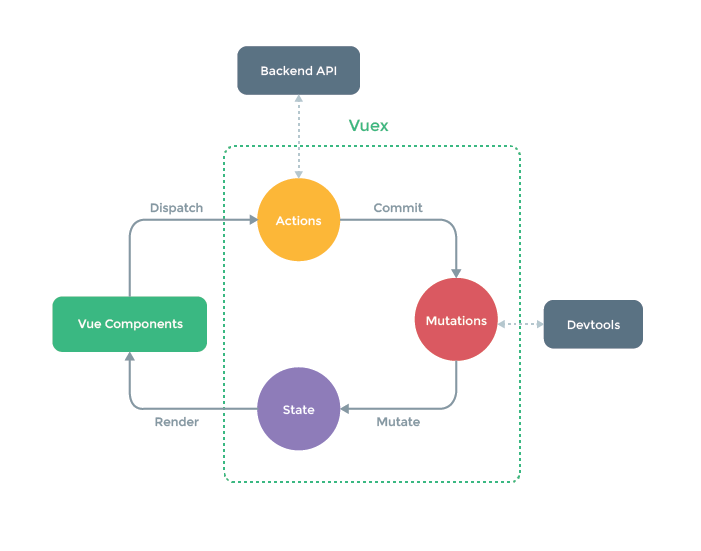
\includegraphics[width=\textwidth]{figures/vuex}
\caption{Schemat przepływu danych w Vuex.}\label{rys:vuex}
\end{figure}

\subsection{Jest}
W projekcie wykorzystano framework testowy Jest~\cite{jest} będący częścią Vue Test Utils. Vue Test Utils to zestaw funkcjonalności upraszczających testowanie komponentów Vue.js. Zestaw ten zapewnia metody umożliwiające symulowanie działań użytkownika w aplikacji oraz przechwytywanie i porównywanie rezultatów tych interakcji z oczekiwanymi. Jest cechuje brak konieczności konfiguracji, izolacja testów oraz szybkość i bezpieczeństwo działania.
\subsection{Json Web Tokens}
Json Web Token~\cite{jwt} jest otwartym standardem przesyłania zabezpieczonych danych. Dane w formacie Json są podpisywane cyfrowo co umożliwia weryfikacje uprawnień. W aplikacjach internetowych JWT stosowane są głownie do autoryzacji użytkowników oraz zapewnienia bezpieczeństwa przesyłanie informacji pomiędzy frontendem, a backendem. Niewielki rozmiar tokenu sprawia iż możliwe jest przesyłanie go w treści zapytania HTTP lub nawet w jego nagłówku. Ta cecha sprawia również, że token może być przechowywany w pamięci przeglądarki, eliminując konieczność ponownego uwierzytelniania po rozpoczęciu nowej sesji.
\subsection{Postman}
Postman~\cite{postman} jest zestawem narzędzi do testowania API (application programming interface). Zapewnia on możliwość wysyłania zapytań HTTP dowolnego typu oraz podgląd odpowiedzi i kodów błędów, jeśli takie wystąpiły. Główną zaletą Postmana jest możliwość tworzenia kolekcji zapytań, które ułatwiają organizację pracy podczas planowania połączeń pomiędzy częścią frontendową i backendową aplikacji. Dodatkowo narzędzie pozwala na współdzielenie kolekcji z zaproszonymi użytkownikami, co znacząco upraszcza proces testowania manualnego. Poza testowaniem manualnym Postman umożliwia tworzenie automatycznych testów przy pomocy języka JavaScript. Dzięki generatorowi losowych danych możliwa jest symulacja działań nawet kilku tysięcy różnych użytkowników w systemie.
\subsection{Visual Studio Code}
Visual Studio Code~\cite{vscode} jest edytorem kodu, którego głównymi zaletami jest wsparcie dla debugowania, inteligentnego uzupełniania kodu, refaktoryzacji oraz kontroli wersji. Dużą korzyścią płynącą z korzystania z program Visual Studio Code jest dostęp do rozszerzeń, usprawniających pracę z kodem w dowolnym języku programowania. Rozszerzenia zapewniają również wsparcie dla frameworków, w tym Vue.js, najbardziej istotnym dla tej części projektu. Mały rozmiar oraz wysoka wydajność znacznie przyśpieszają korzystanie z aplikacji i sprzyjają intensywnej iteracji rozwiązań.
\subsection{Axios}
Axios~\cite{axios} jest biblioteką języka JavaScript służąca do wykonywania zapytań HTTP z poziomu Node.js lub przeglądarki. W aplikacjach internetowych wykorzystywany jest do uzyskiwania danych z części backendowej aplikacji. Axios bazuje na obietnicach (promise), co pozwala na obsługiwanie akcji asynchronicznie. Biblioteka może być użyta poprzez zwykły Javascript lub framework taki jak Vue.js. W porównaniu z innymi bibliotekami służącymi do wykonywania zapytań HTTP Axios oferuje wsparcie dla starszych przeglądarek, możliwość ustawienia ograniczenia czasowego dla zapytań, ochronę przed CSRF (Cross-Site Request Forgery), a także automatyczną transformację danych JSON.
\subsection{Bootstrap}
Bootstrap~\cite{boot} jest frameworkiem CSS (Cascading Style Sheets) upraszczającym projektowanie interfejsu graficznego aplikacji internetowych. Bootstrap pomaga zapewnić responsywność stron, a więc poprawne ich wyświetlanie na urządzeniach mobilnych. Przed pojawieniem się tego rozwiązania często występowała konieczność przygotowywania oddzielnych stylów dla ekranów o rożnych rozdzielczościach. Dzięki zastosowaniu frameworku elementy strony internetowe zostają przeskalowane i przemieszczone tak, aby pomieścić się na ekranie niezależnie od jego wielkości i proporcji. Dodatkowo Bootstrap pozwala na zastosowanie zaawansowanych komponentów takich jak paski nawigacji, wskaźniki postępu czy miniatury. 

\clearpage
\section{Widoki}
\subsection{Strona główna}
Strona główna~(zob.~rysunek~\ref{rys:main}) aplikacji została stworzona na bazie szablonu Bootstrap o nazwie One Page Wonder(źródło). Zawiera ona krótki opis aplikacji, a także korzyści płynących z wykorzystania jej dla planistów, nauczycieli oraz uczniów. Pasek menu znajdujący się zawsze na górze strony jest stałym elementem aplikacji pojawiającym się w każdym z widoków. Pozwala on na przejście do widoków logowania i rejestracji, a przypadku gdy użytkownik jest już zalogowany na wylogowanie lub przejście do widoku szkoły. 
\begin{figure}[!ht]
\centering
\includegraphics[width=\textwidth]{figures/main}
\caption{Aplikacja internetowa - Strona główna}\label{rys:main}
\end{figure}
\subsection{Widok szkoły}
Widok szkoły~(zob.~rysunek~\ref{rys:school}) pozwala na przejście do dodawania danych potrzebnych do wygenerowania planu, a przypadku gdy plan został już wygenerowany jest również miejscem w którym jest on wyświetlany. Rozkład zajęć jest możliwy do wyświetlenia na trzy sposoby - z podziałem na klasy, nauczycieli lub sale lekcyjne.

\begin{figure}[!ht]
\centering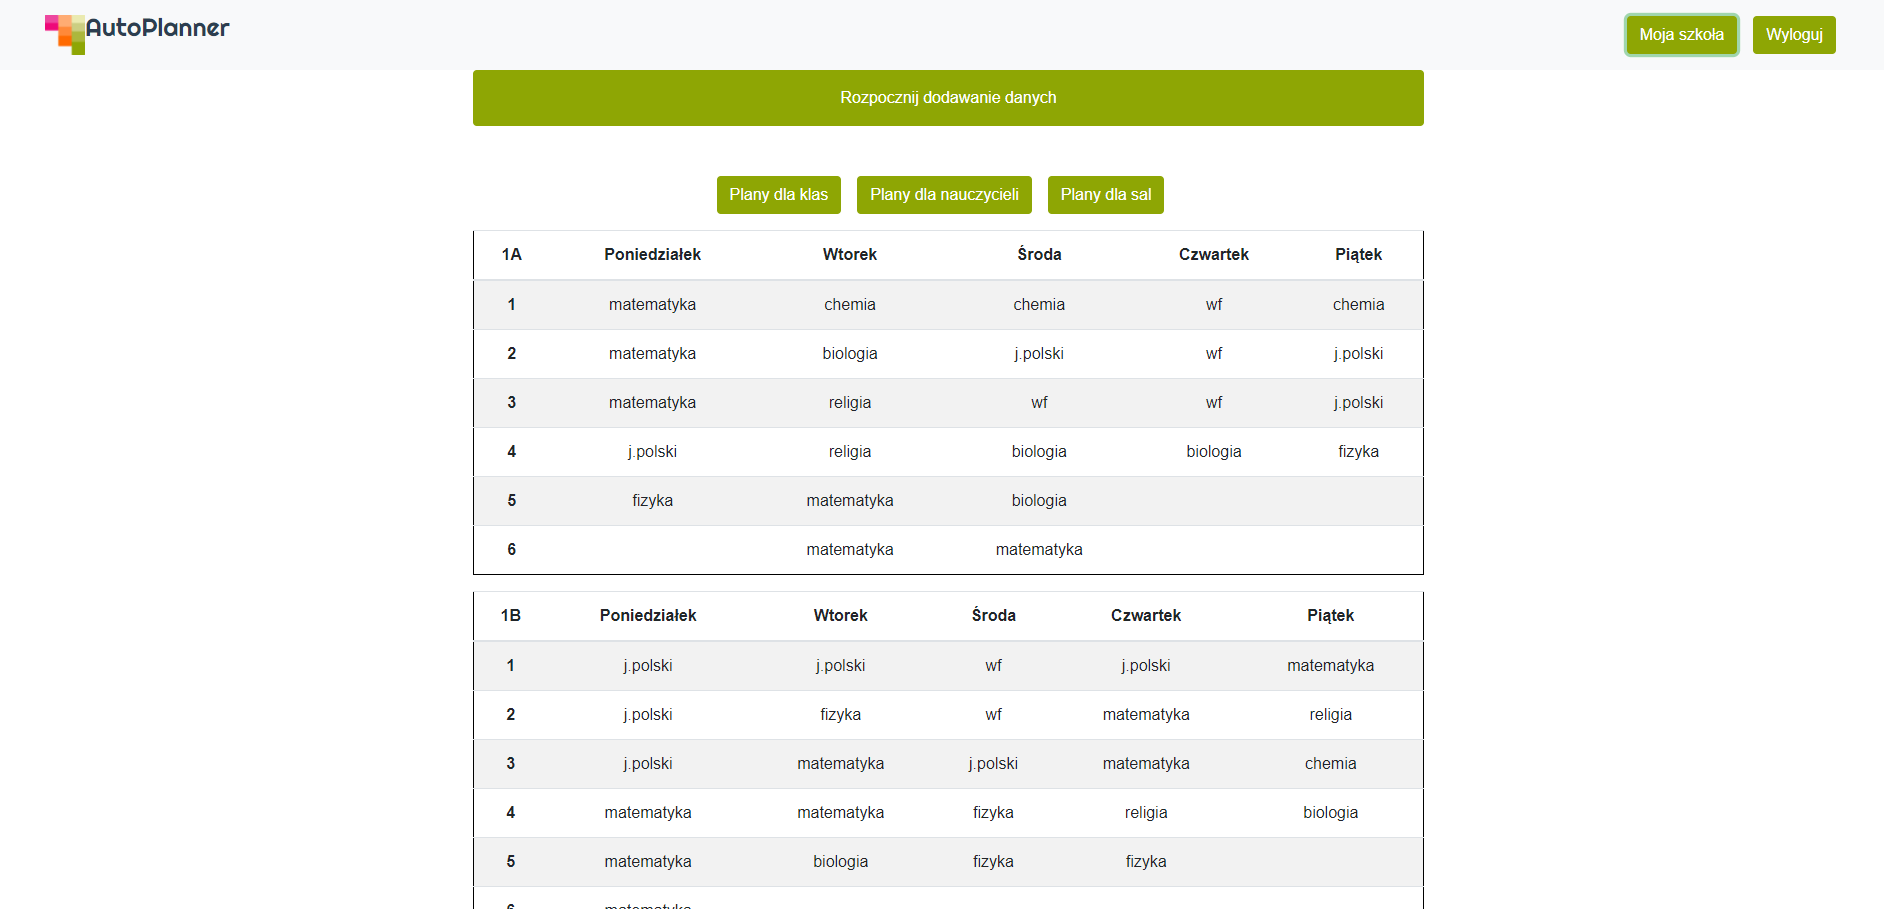
\includegraphics[width=\textwidth]{figures/school}
\caption{Aplikacja internetowa - Widok szkoły}\label{rys:school}
\end{figure}
\subsection{Rejestracja}
Widok rejestracji~(zob.~rysunek~\ref{rys:register}) umożliwia utworzenie konta w serwisie. Od użytkownika wymaga się podania adresu e-mail, nazwy użytkownika oraz hasła. Adres e-mail musi być unikatowy. Wynika to z konieczności weryfikacji konta poprzez wiadomość wysłaną przy pomocy serwera SMTP. Rozwiązanie to ma na celu zapobieganie atakom na stronę poprzez masowe tworzenie nowych kont. 
\begin{figure}[!ht]
\centering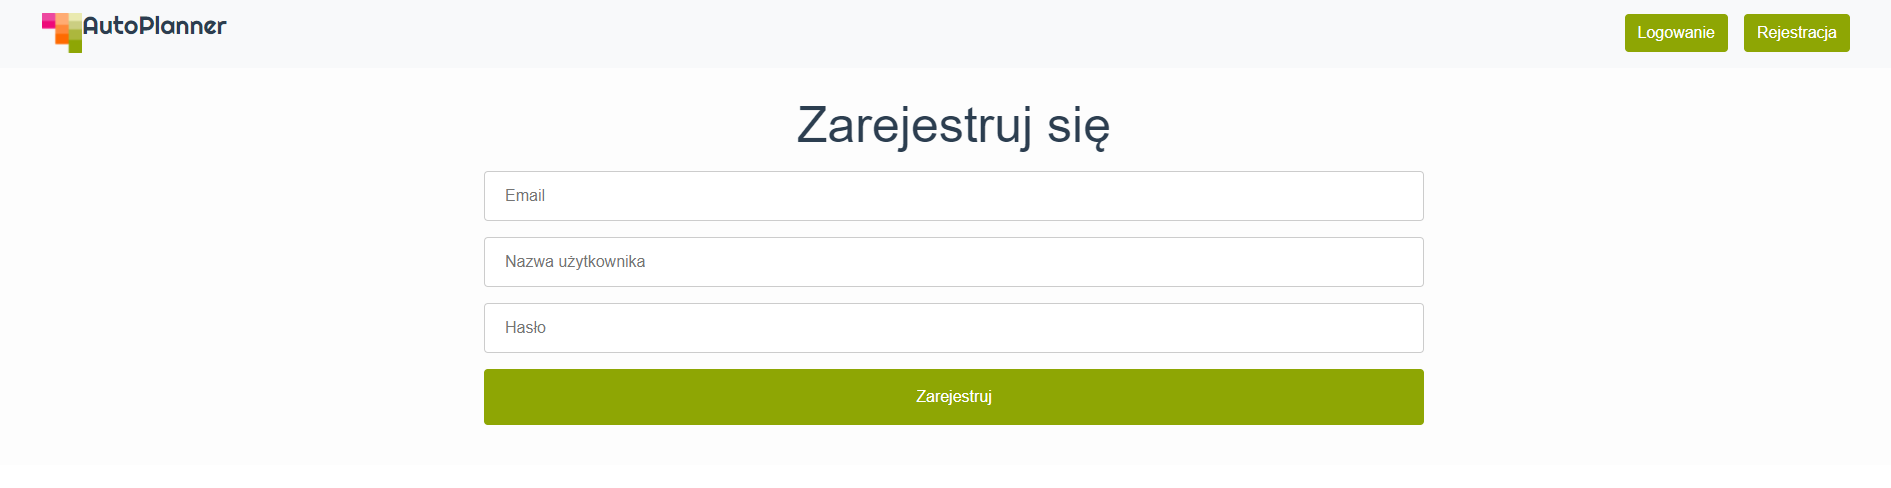
\includegraphics[width=\textwidth]{figures/register}
\caption{Aplikacja internetowa - Widok rejestracji}\label{rys:register}
\end{figure}
\subsection{Logowanie}
Widok logowania~(zob.~rysunek~\ref{rys:login}) pozwala na dostęp do konta i zapisanych na nim danych z dowolnego urządzenia. Do uwierzytelnienia użytkownika wykorzystywany jest adres e-mail oraz hasło podane w procesie rejestracji. Powodzenie procesu logowania powoduje otrzymanie przez aplikację tokenu JWT, zapisywanego w pamięci przeglądarki. W przypadku utraty hasła użytkownik posiada możliwość odzyskania go po podaniu adresu e-mail powiązanego z istniejącym kontem.
\begin{figure}[!ht]
\centering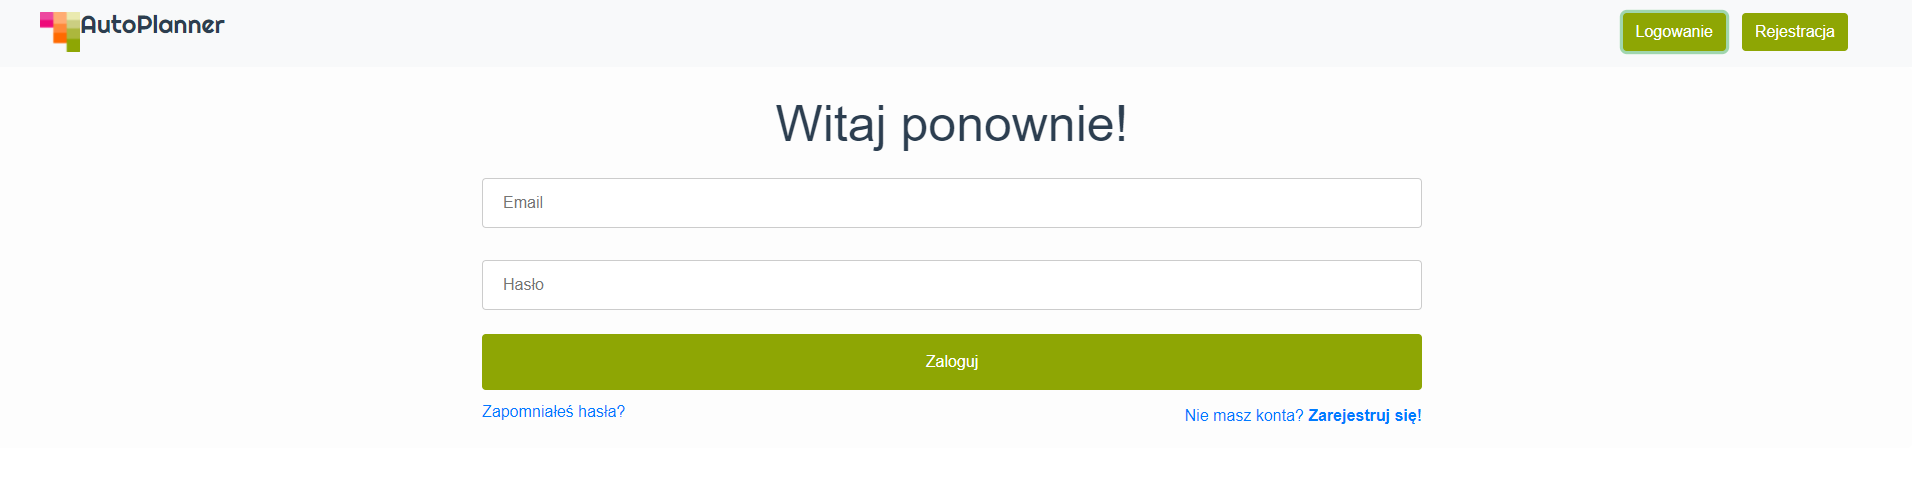
\includegraphics[width=\textwidth]{figures/login}
\caption{Aplikacja internetowa - Widok logowania}\label{rys:login}
\end{figure}
\clearpage
\subsection{Ankieta}
Widok ankiety~(zob.~rysunek~\ref{rys:poll}) pozwala nauczycielowi na podanie preferencji godzinowych pracy. W przeciwieństwie do pozostałych widoków jest on dostępny jedynie poprzez bezpośredni link wysyłany w wiadomości e-mail. Takie rozwiązanie sprawia, że jedynym użytkownikiem, od którego wymagane jest posiadanie konta jest planista. Nauczyciele jako użytkownicy bez konta są identyfikowani dzięki unikalności adresu URL.
\begin{figure}[!ht]
\centering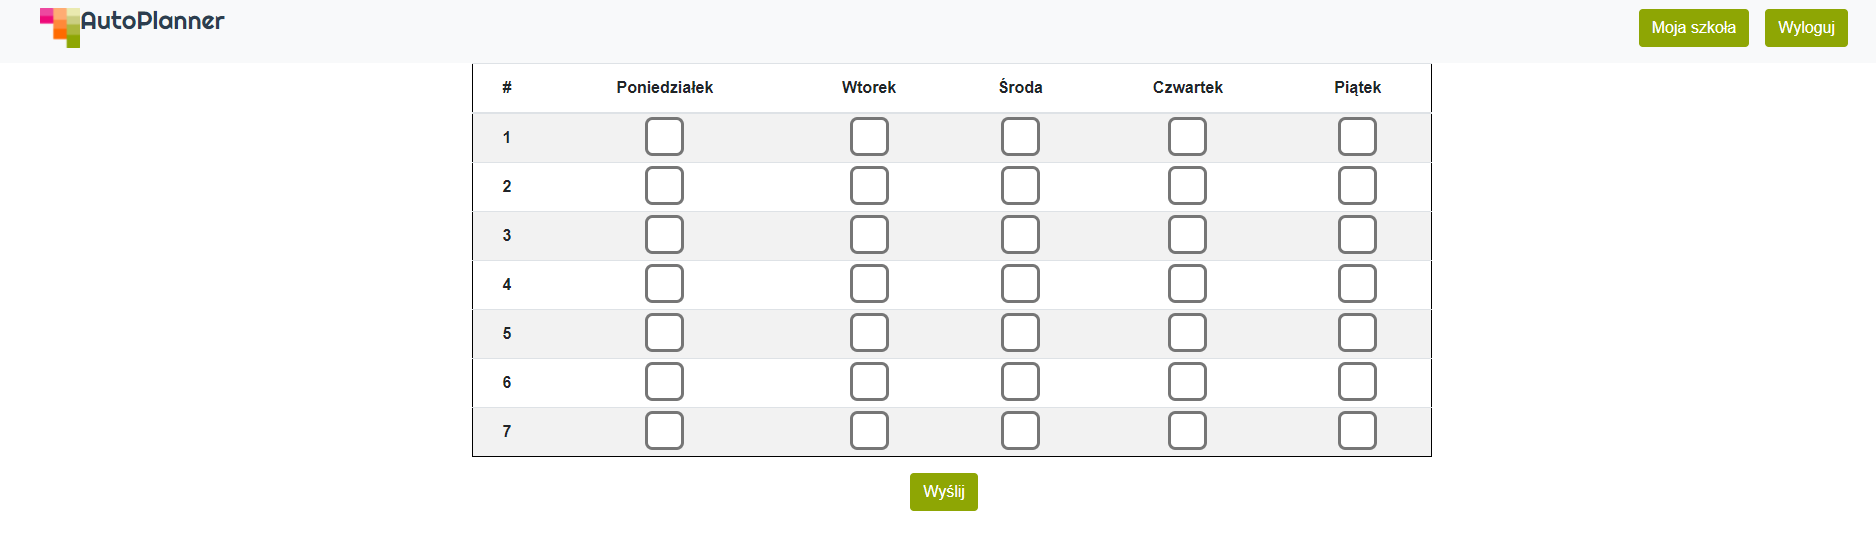
\includegraphics[width=\textwidth]{figures/poll}
\caption{Aplikacja internetowa - Widok ankiet dla nauczycieli}\label{rys:poll}
\end{figure}
\subsection{Dodawanie przedmiotów}
Widok dodawania przedmiotów~(zob.~rysunek~\ref{rys:subject}) stanowi pierwszy krok w procesie podawania danych koniecznych do wygenerowania planu zajęć. W celu dodawania przedmiotu należy podać jedynie jego nazwę. Powiązania z nauczycielami, salami lekcyjnymi i klasami będą mogły być wprowadzone w kolejnych krokach. Podanie nazw przedmiotów na początku procesu dodawania danych pozwala na to, aby w późniejszych etapach mogły być one wybierane z listy rozwijanej. Zapobiega to konieczności wielokrotnego ręcznego wprowadzania tych samych informacji i ułatwia tworzenie powiązań w bazie danych. W lewej części ekranu znajduje się lista już wprowadzonych przedmiotów. Wybranie z nich jednego powoduje przejście do ekranu edycji. Analogiczne rozwiązanie zostało zastosowane we wszystkich kolejnych ekranach dodawania danych.
\begin{figure}[!ht]
\centering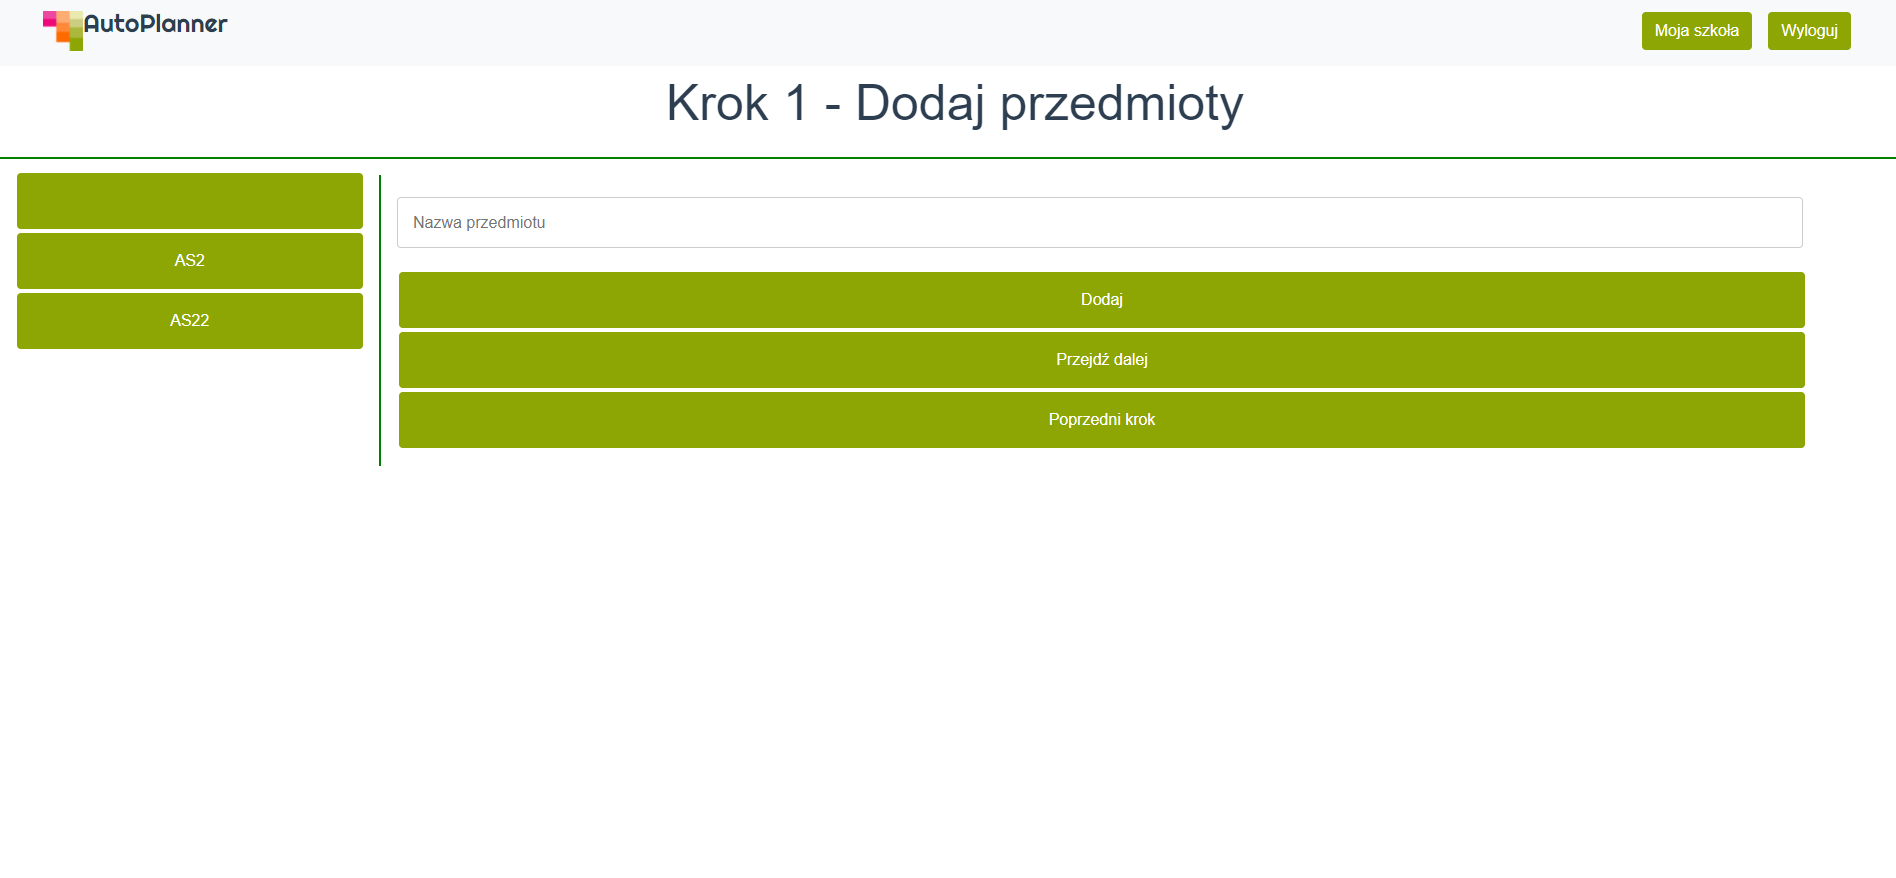
\includegraphics[width=\textwidth]{figures/subject}
\caption{Aplikacja internetowa - Widok dodawania przedmiotów}\label{rys:subject}
\end{figure}
\subsection{Dodawanie nauczycieli}
W widoku dodawania nauczycieli~(zob.~rysunek~\ref{rys:teacher}) planista ma możliwość wprowadzenia danych personelu dydaktycznego oraz jego powiązań z przedmiotami. Każdy nauczyciel musi posiadać imię i nazwisko, unikalny w skali szkoły adres e-mail oraz przynajmniej jeden prowadzony przedmiot. Ekran umożliwia dodanie kolejnych prowadzonych przedmiotów w przypadku, gdy nauczyciel prowadzi więcej niż jeden. 
\begin{figure}[!ht]
\centering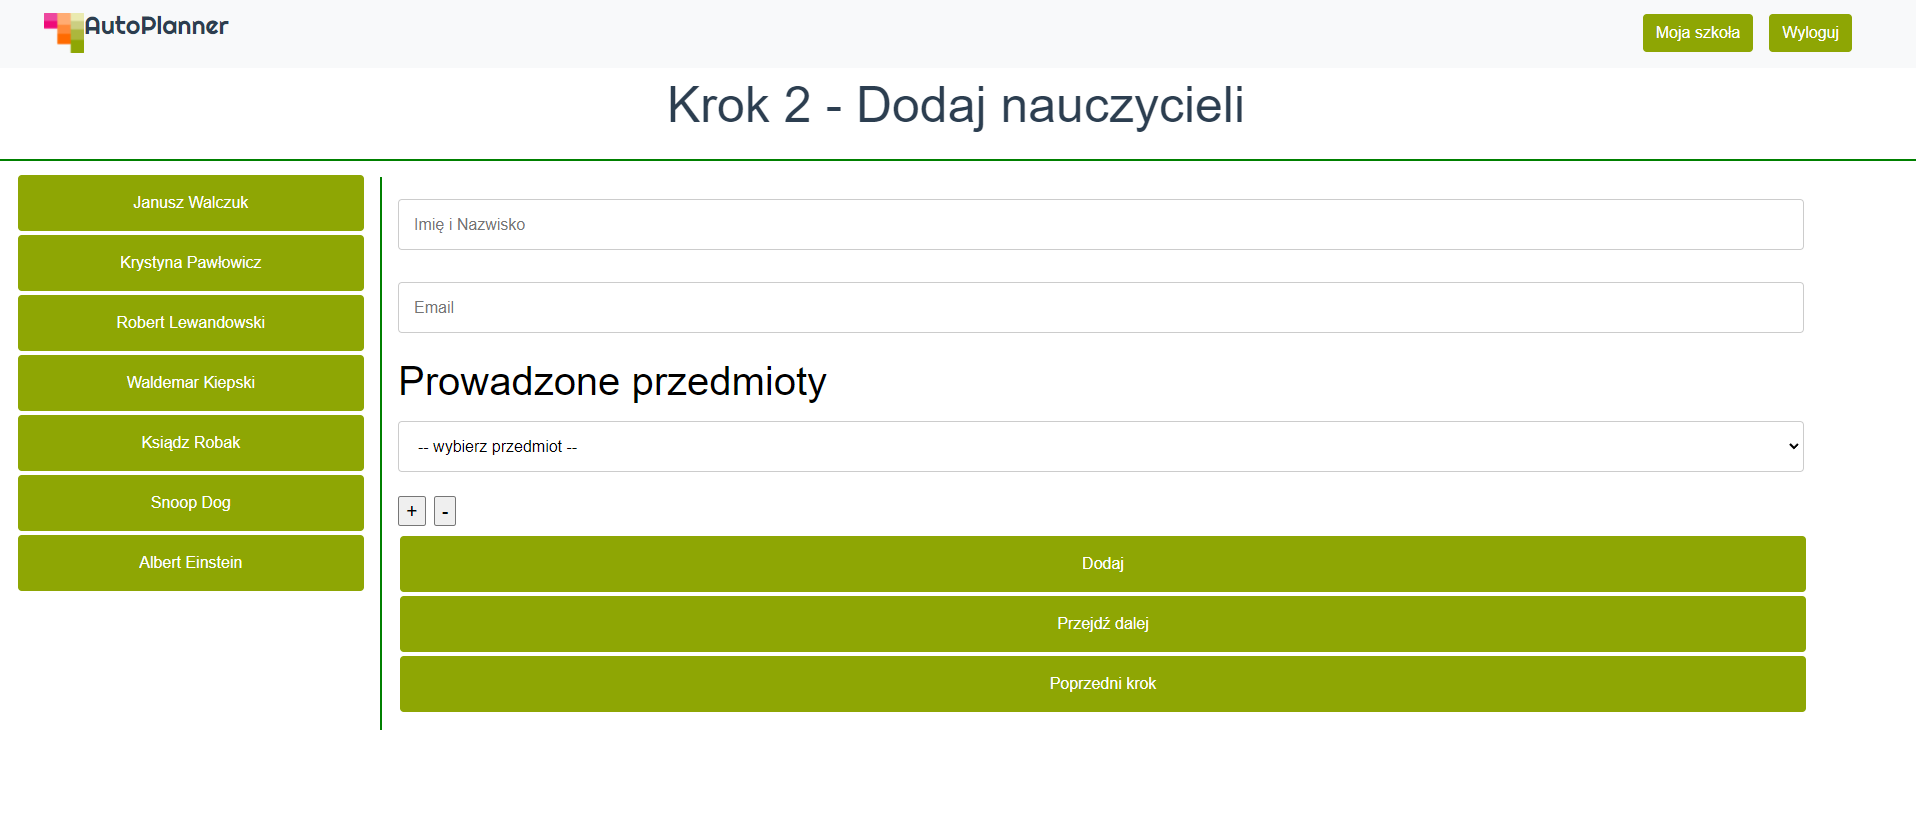
\includegraphics[width=\textwidth]{figures/teacher}
\caption{Aplikacja internetowa - Widok dodawania nauczycieli}\label{rys:teacher}
\end{figure}
\subsection{Dodawanie sali lekcyjnych}
Dodanie informacji o salach lekcyjnych~(zob.~rysunek~\ref{rys:classroom}) stanowi trzeci krok dodawania danych. Sala lekcyjna musi posiadać nazwę, a opcjonalnie także listę przedmiotów, które mogą być w  niej prowadzone. W przypadku, gdy nie zostanie wybrany żaden preferowany przedmiot sala zostaje uznana za salę zwykłą, co oznacza, że będzie mógł być w niej prowadzony dowolny przedmiot.
\begin{figure}[!ht]
\centering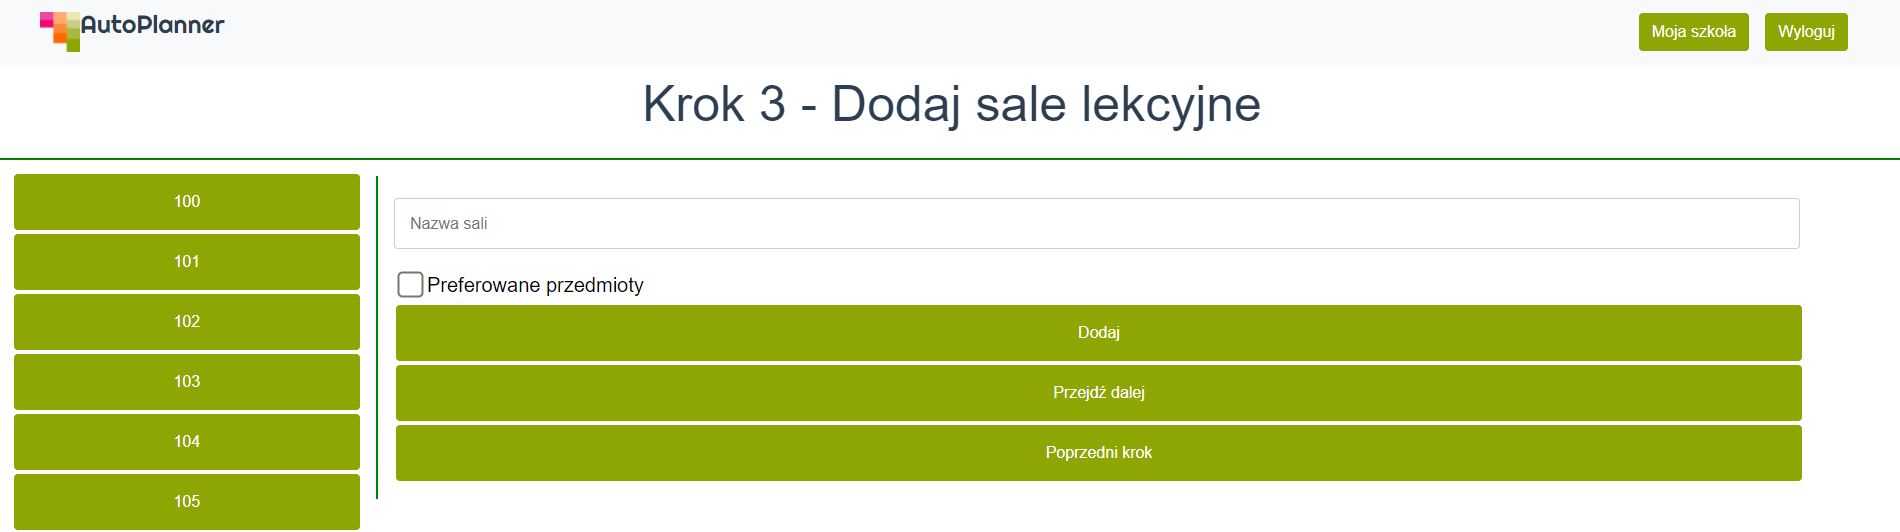
\includegraphics[width=\textwidth]{figures/classroom}
\caption{Aplikacja internetowa - Widok dodawania sali lekcyjnych}\label{rys:classroom}
\end{figure}
\subsection{Dodawanie klas}
Ostatnim etapem w procesie dodawania niezbędnych danych jest wprowadzenie parametrów klas~(zob.~rysunek~\ref{rys:class}). Każda klasa musi posiadać nazwę oraz listę przedmiotów, które mają się pojawić w jej planie zajęć. Każdy element listy musi zawierać nazwę przedmiotu, liczbę godzin lekcyjnych w tygodniu przeznaczonych na przedmiot oraz opcjonalnie prowadzącego przedmiot. Brak wyboru nauczyciela umożliwia przypisanie zajęć dowolnemu prowadzącemu dany przedmiot.
\begin{figure}[!ht]
\centering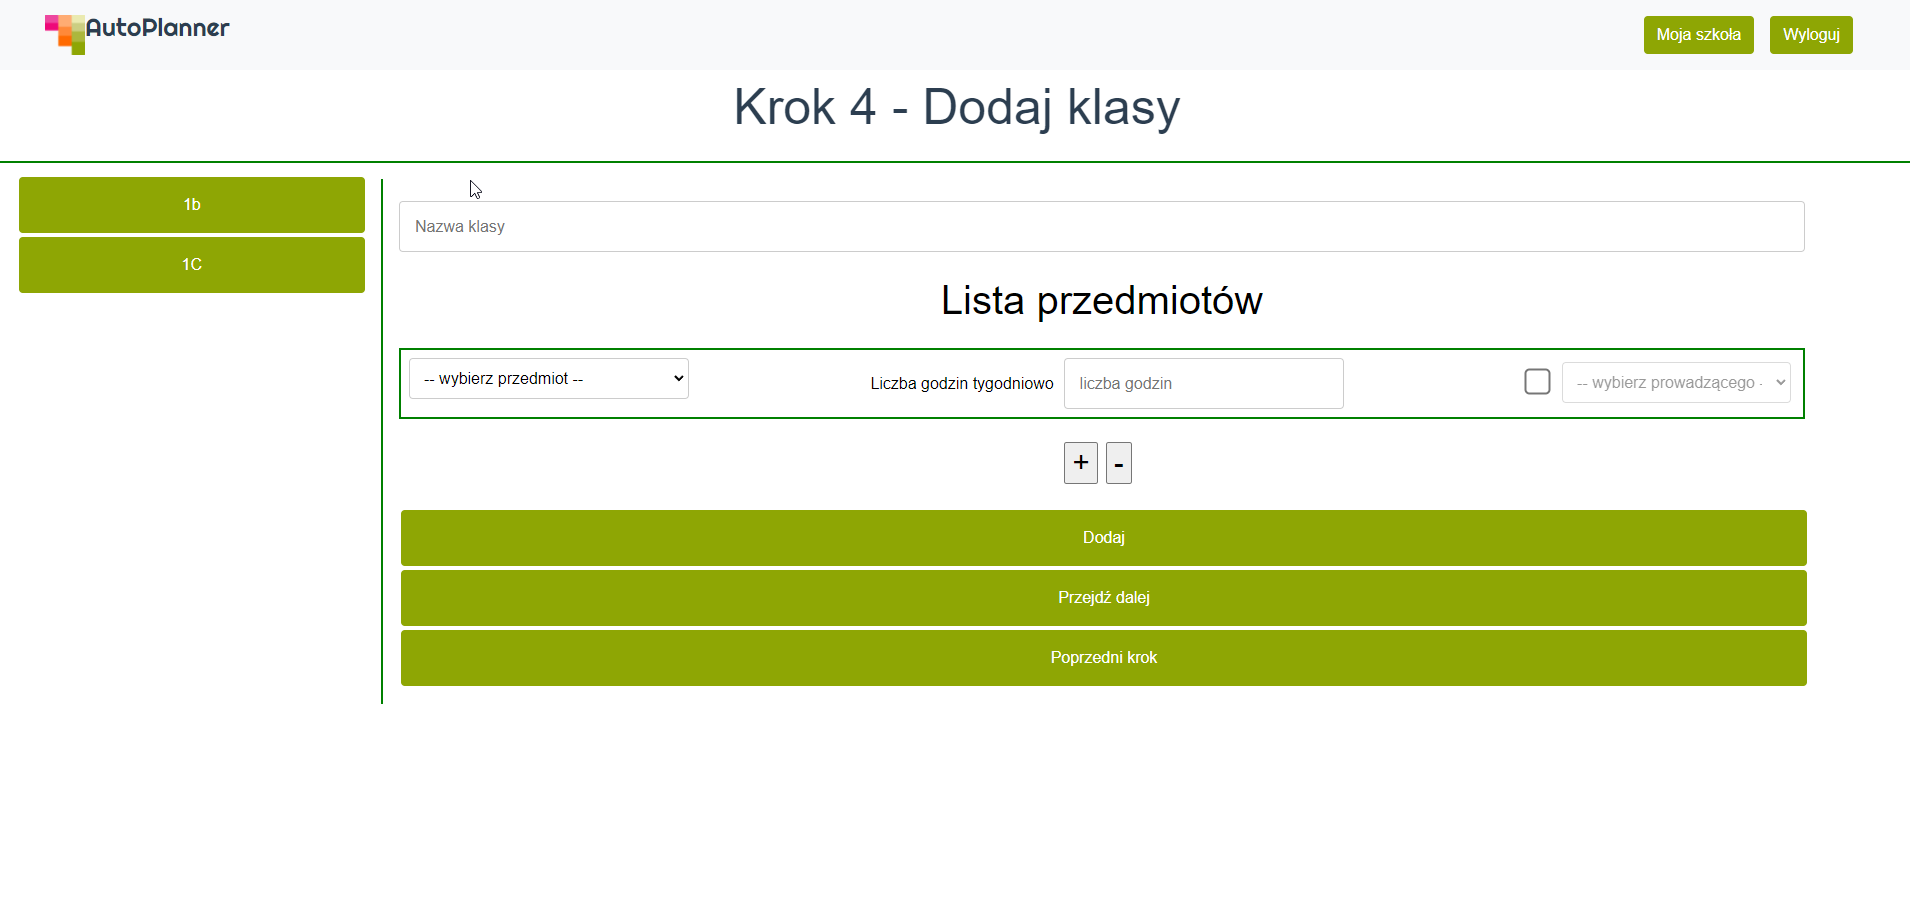
\includegraphics[width=\textwidth]{figures/class}
\caption{Aplikacja internetowa - Widok dodawania klas}\label{rys:class}
\end{figure}
\subsection{Edycja danych}
Dla czterech powyższych ekranów istnieją odpowiadające im ekrany edycji danych. Ze względu na ich analogiczną budowę omówiony zostanie ich struktura zostanie omówiona na bazie widoku edycji danych nauczyciela~(zob.~rysunek~\ref{rys:edit}). Przejście do tego ekranu umożliwiają przyciski znajdujące się po prawej stronie widoku dodawania nauczycieli. Przyciski te są wciąż obecne w widoku edycji i pozwalają na przechodzenie pomiędzy danymi poszczególnych osób bez zapisywania wprowadzonych zmian. W chwili przejścia do ekranu edycji pola z danymi zostają uzupełnione pierwotnie wprowadzonymi informacjami o nauczycielu. Takie rozwiązanie ma celu zapobieganie konieczności ponownego wprowadzania wszystkich danych, w przypadku gdy tylko niektóre z nich wymagają zmian. Przyciski u dołu pozwalają na zapisanie wprowadzonych zmian, powrót do ekranu dodawania nauczycieli lub całkowite usunięcie nauczyciela z bazy danych.
\begin{figure}[!ht]
\centering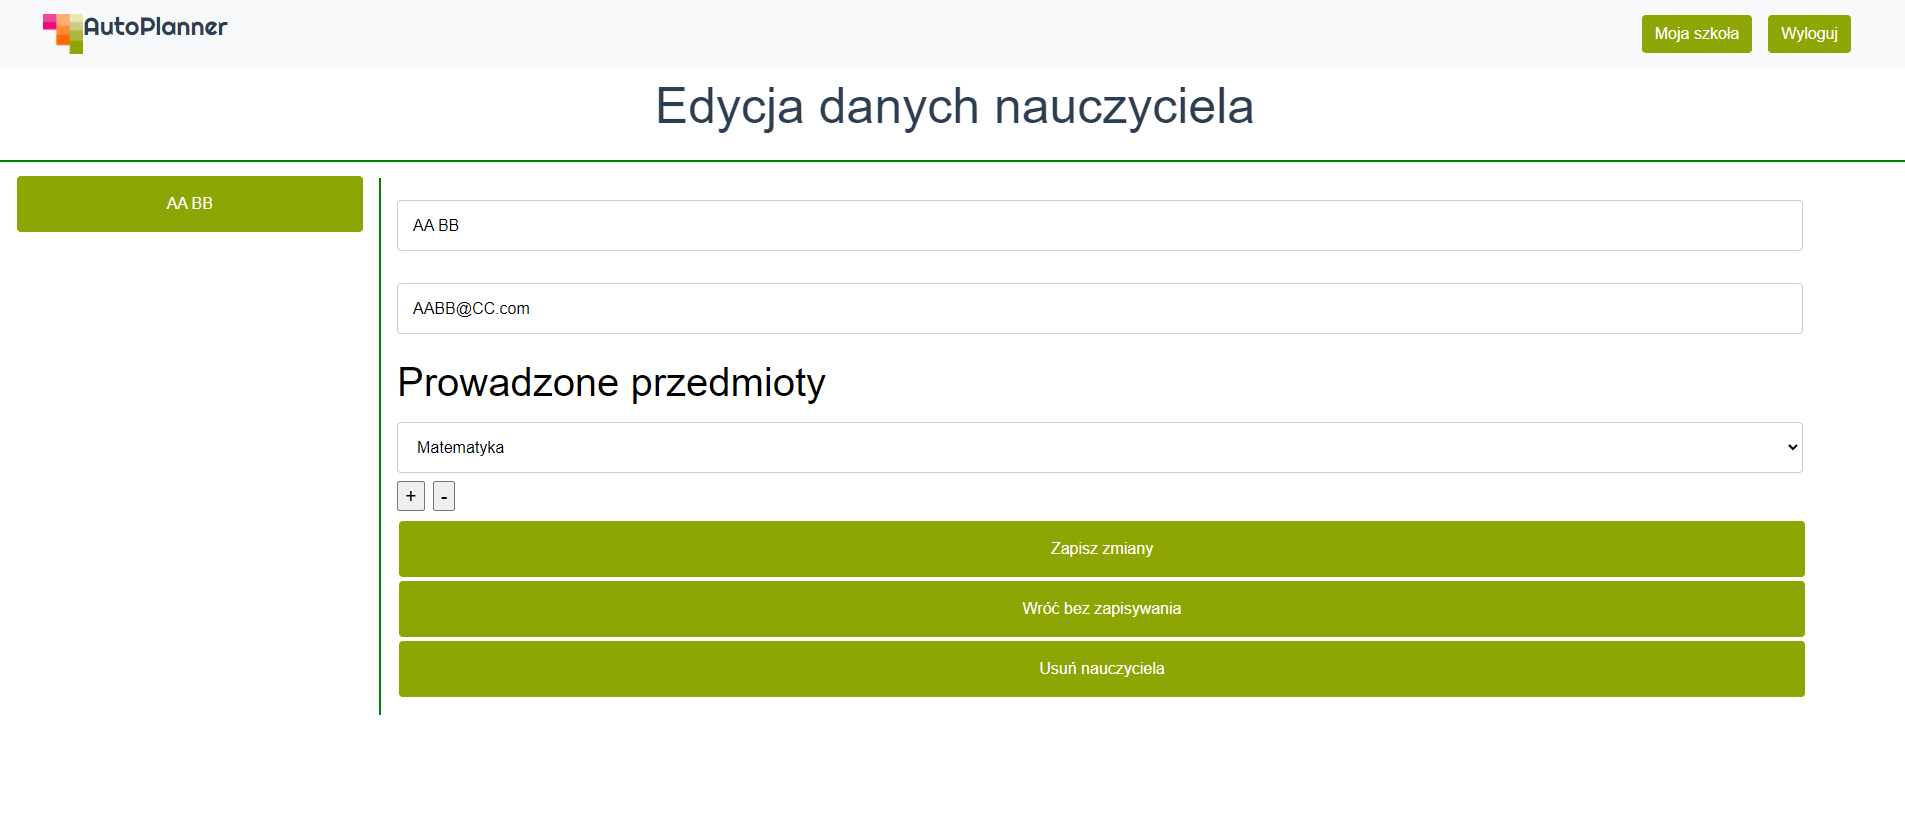
\includegraphics[width=\textwidth]{figures/edit}
\caption{Aplikacja internetowa - Widok edycji danych nauczyciela}\label{rys:edit}
\end{figure}




